\documentclass[11pt,letterpaper,twocolumn]{article}
\usepackage[utf8]{inputenc}
\usepackage[spanish]{babel}
\usepackage{amsmath}
\usepackage{amsfonts}
\usepackage{amssymb}
\usepackage{float}
\usepackage{textcomp}
\usepackage{graphicx}
\usepackage{subfigure}
\usepackage{listings}
\usepackage{verbatim}
\usepackage[left=2cm,right=2cm,top=2cm,bottom=2cm]{geometry}
\begin{document}
\title{\huge{\textbf{ Simulación de un arreglo unidimensional de SRR\textquotesingle  S en MATLAB}}}
\author{\small \textit{M. Sabogal $^{1}$}\\
	\small \textit{ $^{1}$ Programa de Física, Universidad del Atlántico, Km 7 vía a Puerto Colombia, Barranquilla, Colombia}} %Código Postal 081001
\date{} 

\twocolumn[
\begin{@twocolumnfalse}
\maketitle
\begin{center}
{\rule[0mm]{160mm}{0.2mm}}
\end{center}
\begin{abstract}
\textit{Se realizo el estudio y análisis del comportamiento de un modelo no lineal simplificado de un arreglo unidimensional de N resonadores de anillo dividido (SRR\textquotesingle S). Se hayo la relación de dispersión y se comparo con el método de diagonalizacion. También se determinaron las soluciones estacionarias y las familias de soluciones para 2 y 101 SRR\textquotesingle S. Se propagaron las soluciones estacionarias simétrica y asimétrica, observando que en ausencia de efectos disipativos o conducciones extranjeras, la energía se conserva y la solución tiende a mantenerse localizada.\\
\\
\textbf{Palabras claves: SRR, dispersión, disipativos, estacionarias}}
\begin{center}
\textbf{Abstract} 
\end{center}
\par 
\textit{It was carried out the study and analysis of the behavior of a simplified non-linear model of a one-dimensional array of N split-ring resonators (SRR\textquotesingle S). The dispersion relationship was found and compared with the diagonalization method. The stationary solutions and solution families for 2 and 101 SRR\textquotesingle S were also determined. The symmetric and asymmetric stationary solutions were propagated, observing that in the absence of dissipative effects or external conductions, the energy is conserved and the solution tends to remain localized.\\
\\
\textbf{Keywords: SRR, dispersion, dissipative, stationary}}
\end{abstract}
\begin{center}
{\rule[0mm]{160mm}{0.2mm}}
\end{center}
\end{@twocolumnfalse}
]

\section*{\normalsize{INTRODUCCIÓN}} 
En el año de 1967 la propuesta de los materiales con índice de refracción negativo la hizo el físico de la ex Unión Soviética, Victor G. Veselago, quien analizó de forma hipotética el comportamiento de estos materiales, aun cuando sabía que no los podría encontrar en la naturaleza, no fue si no hasta 30 años después que se encontró la posibilidad de construir tales materiales. El principio físico fundamental de estos materiales denominados metamateriales, consiste en sustituir átomos por micro estructuras fabricadas en el laboratorio, las cuales al igual que los átomos, presenten actividad electromagnética, es decir, tienen una función dieléctrica $\varepsilon (w)$ y una magnética $\mu (w)$ $^{[1]}$.\\
\par 
El conocimiento contemporáneo de metamateriales incluye una amplia gama de materiales estructurados artificialmente que exhiben propiedades electromagnéticas y funcionalidades inalcanzables a partir de materiales naturales $[2–5]$. Una clase específica de metamateriales que exhibe propiedades magnéticas significativas en terahercios y frecuencias ópticas está representada por los metamateriales magnéticos (MM) $[6,7]$, que habitualmente se componen de resonadores de anillo dividido (SRR\textquotesingle S)$^{[8]}$. Los bloques de construcción importantes de los metamateriales electromagnéticos $[9]$ son los resonadores de anillo dividido (SRR\textquotesingle S) u otros tipos de elementos resonantes de sublongitud de onda que están dispuestos en redes tridimensionales de una, dos o tres dimensiones. En general, la respuesta de un metamaterial no está dada simplemente por una suma de las respuestas de resonadores individuales, sino que también depende de la interacción de campo cercano entre los resonadores dentro del sistema $[10, 11]$. Un enfoque teórico estándar para analizar las propiedades de los metamateriales se basa en la aproximación efectiva del medio cuando la estructura se trata como un medio homogéneo caracterizado por parámetros macroscópicos efectivos$^{[12]}$. Se desea estudiar con énfasis un modelo no lineal simplificado de un arreglo unidimensional de resonadores de anillo dividido (SRR\textquotesingle S), a partir de simulaciones computacionales en MATLAB. 
\subsection*{SRR}
Un SRR de celda única tiene un par de bucles cerrados con divisiones en los extremos opuestos. Los bucles están hechos de metal no magnético como el cobre y tienen un pequeño espacio entre ellos. Los bucles pueden ser concéntricos, o cuadrados, y estar separados según sea necesario. Un flujo magnético que penetre en los anillos metálicos inducirá corrientes giratorias en los anillos, que producen su propio flujo para mejorar u oponerse al campo incidente (dependiendo de las propiedades resonantes de los SRR). Este patrón de campo es dipolar. Los pequeños espacios entre los anillos producen grandes valores de capacitancia que disminuyen la frecuencia de resonancia.$^{[13]}$ \\

En su versión más simple, un SRR es solo un anillo metálico con una ranura, donde se forma una capacitancia C. Bajo ciertas condiciones, puede tratarse como un circuito RLC en serie, que presenta una resonancia inductiva-capacitiva a $\omega_{r}=1/\sqrt{LC}$, con $L$ siendo la autoinductancia del SRR y suponiendo que las pérdidas óhmicas son bajas.$^{[8]}$
\subsection*{Modelo no lineal}
Un SRR se vuelve no lineal ya sea mediante la inserción de un dieléctrico no lineal $[14]$ o un diodo Varicap ( diodo de capacidad variable)  $[15,16,17]$ en su ranura. Ambas formas dan como resultado una capacitancia SRR dependiente de voltaje que puede ser aproximada por una no linealidad cúbica. La construcción de una serie de SRR no lineales, que están débilmente acopladas a través de interacciones magnéticas $[18,19,20]$ da como resultado un MM sintonizable no lineal $[15]$. Considere una matriz 1D como se observa en la figura $(1)$, donde todos los SRR tienen la misma frecuencia de resonancia $\omega_{o}$: \\
\begin{figure}[h!]
\centering 
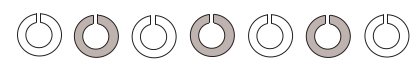
\includegraphics[scale=0.45]{srr.png}
\caption{Arreglo unidimensional de SRR\textquotesingle S. Obtenido de $[21]$}
\end{figure}
\par 
Ésta matriz binaria no lineal se coloca en un campo magnético alternante perpendicular a los planos de los SRR. Luego, la ecuación dinámica normalizada para la carga $q_{n}$ acumulada en el condensador del enésimo SRR es$^{[8]}$:\\
{\fontsize{9}{15}\selectfont
\begin{equation}
\dfrac{d^{2}}{dt^{2}} \left[ q_{n} + \lambda \left( q_{n+1} + q_{n-1}\right) \right] + \gamma \dfrac{d q_{n}}{dt}+ \omega_{o}^{2} q_{n} - \chi \omega_{o}^{6} q_{n}^{3}= \varepsilon_{0} \sin(\hat{\omega}t)
\end{equation} }
\par 
Donde $\lambda$ es el parámetro de acoplamiento ($\lambda > 0$ en el presente modelo), $\gamma$ es el coeficiente de pérdida, $\chi$ es el parámetro de no linealidad, y el término en el lado derecho de la ecuación es la fuerza electromotriz de frecuencia inducida en cada SRR debido al campo aplicado.
\subsection*{Modelo no lineal simplificado}
A partir del modelo de la ecuacion $(1)$ se toman las consideraciones $\gamma=0$ y $ \varepsilon_{0}=0$,  obtiendo la ecuación dinámica normalizada para la carga $q_{n}$ acumulada en el condensador del enésimo SRR, sin efectos de perdida y sin fuerza electromotriz de frecuencia inducida:\\
\begin{equation}
\dfrac{d^{2}}{dt^{2}} \left[ q_{n} + \lambda \left( q_{n+1} + q_{n-1}\right) \right] + \omega_{o}^{2} q_{n} - \chi \omega_{o}^{6} q_{n}^{3}=0
\end{equation}
\par 
Es decir sin disipación y conducción externa. La ecuación anterior puede se obtener del hamiltoniano, donde la densidad Hamiltoniana discreta $H= \sum_{n} H_{n}$ viene dada por: 
\begin{equation}
H_{n}= \dfrac{1}{2}\left[ \dot{q}_{n}^{2} + \dot{q}_{n}\left(\dot{q}_{n-1}+\dot{q}_{n+1}\right) \right] + V_{n}
\end{equation}
\par  
Donde $V_{n}$ es el potencial no lineal del enésimo termino.
$$V_{n}=\dfrac{1}{2}\left(\omega_{o} q_{n}\right)^{2} \left[ 1- \dfrac{1}{2}\chi \left(\omega_{o}^{2}q_{n}\right)^{2} \right]$$
\par 
El Hamiltonian $H$ es en realidad la energía conservada del sistema sin pérdidas en ausencia de cualquier sistema de términos de conducción.
\subsubsection*{Relación de dispersión}
Tomando el caso lineal de la ecuacion $(2)$, es decir $\chi=0$, se tiene:
\begin{equation}
\dfrac{d^{2}}{dt^{2}} \left[ q_{n} + \lambda \left( q_{n+1} + q_{n-1}\right) \right] + \omega_{o}^{2} q_{n} = 0 
\end{equation}
Suponiendo la solucion de la forma: 
$$q_{n}(t)=Q_{n} \exp(i \Omega t)$$
Remplazando y agupando: 
\begin{equation}
\Omega^{2} \left[ Q_{n} + \lambda Q_{n-1} + \lambda Q_{n+1}\right]=\omega_{o}^{2}Q_{n}
\end{equation}
Tomando soluciones estacionarias $Q_{n}=A\exp(ikn)$ donde $0<k<\pi$ : 
remplazando y operando se obtiene: 
$$\Omega^{2} \left[ 1 + \lambda \exp(-ik)+\lambda \exp(ik) \right] = \omega_{o}^{2}$$
Utilizando la expresion de euler para el coseno: 
$$\Omega^{2} \left[ 1 + 2 \lambda \cos(k) \right] = \omega_{o}^{2} $$
Obtiendo la relacion de dispersión para el caso lineal:  
\begin{equation}
\Omega= \pm \dfrac{\omega_{o}}{\sqrt{1 + 2 \lambda \cos(k)}}
\end{equation}
De igual forma, una manera analoga para determinar estos valores es escribiendo la ecuacion $(5)$, de manera matricial para el sistema de $N$ resonadores. 
{\fontsize{7}{15}\selectfont
$$ \Omega^{2} \left(
\begin{matrix}
1 & \lambda  & 0 & 0 & 0 & \cdots & 0 & 0 \\
\lambda & 1 & \lambda  & 0 & 0 & \cdots & 0 & 0\\
0 & \lambda  & 1 & \lambda   & 0 & \cdots & 0& 0 \\
0 & 0 & \lambda  & 1 & \lambda   & \cdots & 0 & 0 \\
\vdots & \vdots & \vdots & \ddots & \ddots & \ddots & \vdots & \vdots \\
0 & 0 & 0 & \cdots & \lambda  &  1 & \lambda &0\\    
0 & 0 & 0 & \cdots & 0 & \lambda  & 1 & \lambda\\    
0 & 0 & 0 & \cdots & 0 & 0 & \lambda  & 1    
\end{matrix} \right) \left(
\begin{matrix}
Q_{1}\\
Q_{2}\\
Q_{3}\\
Q_{4}\\
\vdots\\
Q_{n-3}\\
Q_{n-2}\\
Q_{n-1}\\
Q_{n}
\end{matrix} \right) =\omega_{o}^{2} \left(
\begin{matrix}
Q_{1}\\
Q_{2}\\
Q_{3}\\
Q_{4}\\
\vdots\\
Q_{n-3}\\
Q_{n-2}\\
Q_{n-1}\\
Q_{n}
\end{matrix} \right)
$$}
Rescribiendo lo anterior de la forma: 
$$\Omega^{2} \hat{M} \vec{Q} = \omega_{o}^{2} \vec{Q}$$
Despejando: 
\begin{equation}
\omega_{o}^{2} \hat{M}^{-1} \vec{Q}=\Omega^{2} \vec{Q}
\end{equation}
Obtiendo un problema de valos propios, donde $\Omega^{2}$ seran los valores propios de la matriz $\hat{W}=\omega_{o}^{2} \hat{M}^{-1}$. 
\subsubsection*{Soluciones estacionarias}
Para las soluciones estacionarias del problema no lineal, se toman soluciones armonicas para el modelo de la ecuacion $(2)$: 
$$q_{n}(t)=Q_{n} \sen(\Omega t)$$
Derivando y remplazando: 
$$\left( \omega_{o}^{2} - \Omega^{2} \right) Q_{n} \sen(\Omega t) + \chi \omega_{o}^{6} Q_{n}^{3} \sen^{3}(\Omega t)-$$ 
$$ \Omega^{2} \lambda \left( Q_{n-1} + Q_{n+1} \right) \sen(\Omega t)=0 $$
Utilizando la aproximacion de onda rotante $\sen^{3}(x)=3/4 \sen(x)$ se obtiene para el n-esimo resonador: 
$$\dfrac{3}{4}\chi\omega_{o}^{6}Q_{n}^{3} + \left( \Omega^{2}-\omega_{o}^{2} \right) Q_{n} + \lambda \Omega^{2} \left( Q_{n-1} + Q_{n+1} \right) =0$$
Escribiendo el sistema algebraico de $n$ ecuaciones no linales de forma matricial, cuyas soluciones son las $Q_{n}$ estacionarias: 
{\fontsize{3}{15}\selectfont
\begin{equation}
\left(
\begin{matrix}
a+bQ_{1}^{2} & \lambda \Omega^{2} & 0 & 0 & \cdots & 0 & 0 \\
\lambda \Omega^{2} & a+bQ_{2}^{2} &  \lambda\Omega^{2} & 0 & \cdots & 0 & 0\\
0 & \lambda \Omega^{2} & a+bQ_{3}^{2} & \lambda \Omega^{2}  & \cdots & 0& 0 \\

\vdots & \vdots & \ddots & \ddots & \ddots & \vdots & \vdots \\
0 & 0 & \cdots & \lambda \Omega^{2} &  a+bQ_{n-2}^{2} & \lambda \Omega^{2} &0\\    
0 & 0 & \cdots & 0 & \lambda \Omega^{2} & a+bQ_{n-1}^{2} & \lambda \Omega^{2}\\    
0 & 0 & \cdots & 0 & 0 & \lambda \Omega^{2}  & a+bQ_{n}^{2}     
\end{matrix} \right) \left(
\begin{matrix}
Q_{1}\\
Q_{2}\\
Q_{3}\\
\vdots\\
Q_{n-2}\\
Q_{n-1}\\
Q_{n}
\end{matrix} \right)= \left(
\begin{matrix}
0\\
0\\
0\\
\vdots\\
0\\
0\\
0
\end{matrix} \right)
\end{equation}
} 
Donde $a=\left( \Omega^{2}-\omega_{o}^{2} \right)$ y $b=\dfrac{3}{4}\chi\omega_{o}^{6}$
\subsubsection*{Propagacion de las soluciones}
Retomando nuevamente la ecuación ecuacion $(2)$ para el énesimo resonador acoplado: 
$$\dfrac{d^{2}}{dt^{2}} \left[ q_{n} + \lambda \left( q_{n+1} + q_{n-1}\right) \right] = - \omega_{o}^{2} q_{n} + \chi \omega_{o}^{6} q_{n}^{3} $$
\par 
Para $n=1,2,3,4 \cdots n$; donde $q_{n+1}=0$, se tiene el sistema en el lado derecho de la ecuacion $1$:
{\fontsize{9}{15}\selectfont
$$\dfrac{d^{2}}{dt^{2}} \left(
\begin{matrix}
q_{1} & \lambda q_{2} & 0 & 0 & 0 & \cdots & 0 & 0 \\
\lambda q_{1} & q_{2} & \lambda q_{3} & 0 & 0 & \cdots & 0 & 0\\
0 & \lambda q_{2} & q_{3} & \lambda q_{4}  & 0 & \cdots & 0& 0 \\
0 & 0 & \lambda q_{3} & q_{4} & \lambda q_{5}  & \cdots & 0 & 0 \\
\vdots & \vdots & \vdots & \ddots & \ddots & \ddots & \vdots & \vdots \\
0 & 0 & 0 & \cdots & \lambda q_{n-3} &  q_{n-2} & \lambda q_{n-1} &0\\    
0 & 0 & 0 & \cdots & 0 & \lambda q_{n-2} & q_{n-1} & \lambda q_{n}\\    
0 & 0 & 0 & \cdots & 0 & 0 & \lambda q_{n-1} & q_{n}     
\end{matrix} \right) = $$
$$=  \dfrac{d^{2}}{dt^{2}} \left[ 
\left(
\begin{matrix}
1 & \lambda  & 0 & 0 & 0 & \cdots & 0 & 0 \\
\lambda & 1 & \lambda  & 0 & 0 & \cdots & 0 & 0\\
0 & \lambda  & 1 & \lambda   & 0 & \cdots & 0& 0 \\
0 & 0 & \lambda  & 1 & \lambda   & \cdots & 0 & 0 \\
\vdots & \vdots & \vdots & \ddots & \ddots & \ddots & \vdots & \vdots \\
0 & 0 & 0 & \cdots & \lambda  &  1 & \lambda &0\\    
0 & 0 & 0 & \cdots & 0 & \lambda  & 1 & \lambda\\    
0 & 0 & 0 & \cdots & 0 & 0 & \lambda  & 1    
\end{matrix} \right) \left(
\begin{matrix}
q_{1}\\
q_{2}\\
q_{3}\\
q_{4}\\
\vdots\\
q_{n-3}\\
q_{n-2}\\
q_{n-1}\\
q_{n}
\end{matrix} \right) \right]$$
}
\par 
Debido a la linealidad de los operadores involucrados es posible reescribir la expresion de la forma: 
{\fontsize{8}{15}\selectfont
\begin{equation}
\left(
\begin{matrix}
1 & \lambda  & 0 & 0 & 0 & \cdots & 0 & 0 \\
\lambda & 1 & \lambda  & 0 & 0 & \cdots & 0 & 0\\
0 & \lambda  & 1 & \lambda   & 0 & \cdots & 0& 0 \\
0 & 0 & \lambda  & 1 & \lambda   & \cdots & 0 & 0 \\
\vdots & \vdots & \vdots & \ddots & \ddots & \ddots & \vdots & \vdots \\
0 & 0 & 0 & \cdots & \lambda  &  1 & \lambda &0\\    
0 & 0 & 0 & \cdots & 0 & \lambda  & 1 & \lambda\\    
0 & 0 & 0 & \cdots & 0 & 0 & \lambda  & 1    
\end{matrix} \right) \dfrac{d^2}{dt^2} \left(
\begin{matrix}
q_{1}\\
q_{2}\\
q_{3}\\
q_{4}\\
\vdots\\
q_{n-3}\\
q_{n-2}\\
q_{n-1}\\
q_{n}
\end{matrix} \right)  = \hat{M_{1}} \dfrac{d^{2} \vec{q}_{n}}{dt^{2}}
\end{equation} } 
De manera similar para el lado derecho de la ecuacion $(2)$, se tiene el sistema: 
{\fontsize{8}{15}\selectfont
$$ \left(
\begin{matrix}
- \omega_{o}^{2} q_{1} + \chi \omega_{o}^{6} q_{1}^{3} & 0 & \cdots & 0 \\
0  & - \omega_{o}^{2} q_{2} + \chi \omega_{o}^{6} q_{2}^{3} & \cdots & 0 \\
\vdots & \vdots  & \ddots & \vdots & \\
0 & 0 & \cdots &- \omega_{o}^{2} q_{n} + \chi \omega_{o}^{6} q_{n}^{3}\\     
\end{matrix} \right) = $$ }
{\fontsize{6}{15}\selectfont
\begin{equation}
\left(
\begin{matrix}
- \omega_{o}^{2} + \chi \omega_{o}^{6} q_{1}^{2} & 0 & \cdots & 0 \\
0  & - \omega_{o}^{2} + \chi \omega_{o}^{6} q_{2}^{2} & \cdots & 0 \\
\vdots & \vdots  & \ddots & \vdots & \\
0 & 0 & \cdots &- \omega_{o}^{2} + \chi \omega_{o}^{6} q_{n}^{2}\\     
\end{matrix} \right) \left( \begin{matrix}
q_{1}\\
q_{2}\\
\vdots\\
q_{n}
\end{matrix} \right) = \hat{M_{2}} \vec{q}_{n}
\end{equation}
}
Igualando $9$ y $10$ se obtiene: 
$$\hat{M_{1}} \dfrac{d^{2} \vec{q}_{n}}{dt^{2}} = \hat{M_{2}} \vec{q}_{n} \hspace*{0.3 cm} \rightarrow \hspace*{0.3 cm}\dfrac{d^{2} \vec{q}_{n}}{dt^{2}} = \hat{M_{1}^{-1}} \hat{M_{2}} \vec{q}_{n} $$
\begin{equation}
\dfrac{d^{2} \vec{q}_{n}}{dt^{2}}=\hat{M_{3}} \vec{q}_{n}
\end{equation}
\par 
Donde $\hat{M_{3}}=\hat{M_{1}^{-1}} \hat{M_{2}}$, reduciendo el sistema a un problema de valores propios, tomando la observación de que la matriz $\hat{M_{3}}$ cambia en el tiempo debido a los terminos no lineales  presentes en la matriz $\hat{M_{2}}$.
\section*{-Implementación, interpretación física y resultados}
Con el fin de estudiar el comportamiento del modelo no lineal simplificado de un arreglo unidimensional de resonadores de anillo dividido (SRR\textquotesingle S) y sus características, se realizaron diferentes simulaciones del modelo, para $N=2$ osciladores y $N=101$ mediante las herramientas computacionales de MATLAB.\\
\par 
En primera instancia se observo la relación de dispersión en la figura $2$ (a), obtenida en la ecuación ($6$), en la que se observa el gap, donde se encuentran las soluciones no lineales. De igual forma se observa el la figura $2$ (b) que el sistema de diagonalización propuesto en la ecuación ($7$), el cual se resolvió utilizando la funcion \textit{eig()}, es análogo al de la ecuación ($6$) para determinar los valores propios del sistema lineal. \\  
\begin{figure}[h!]
\centering
\subfigure[] {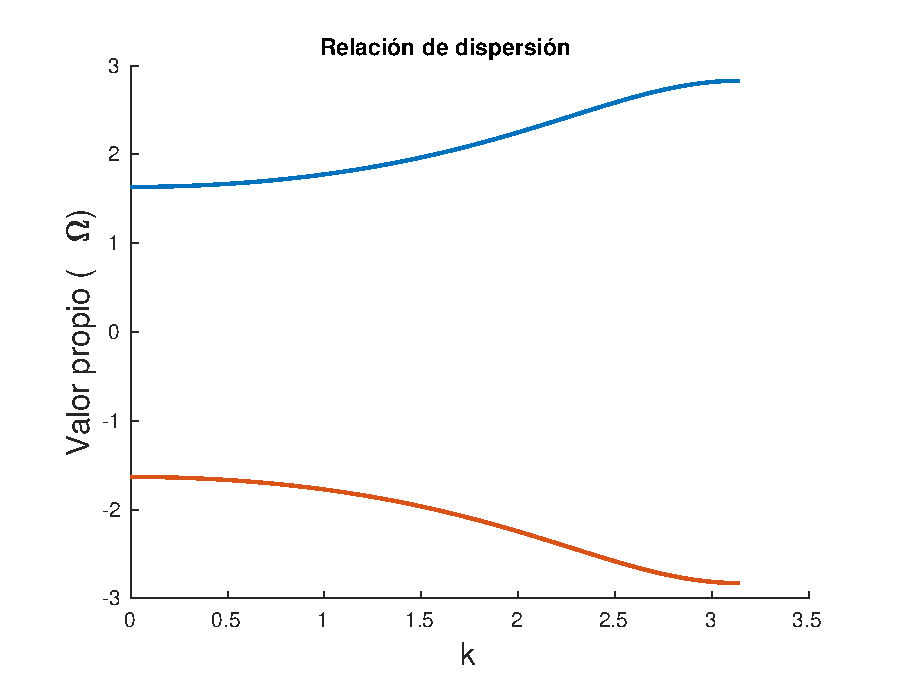
\includegraphics[scale=0.46]{RDSP-T.eps}}
\subfigure[] {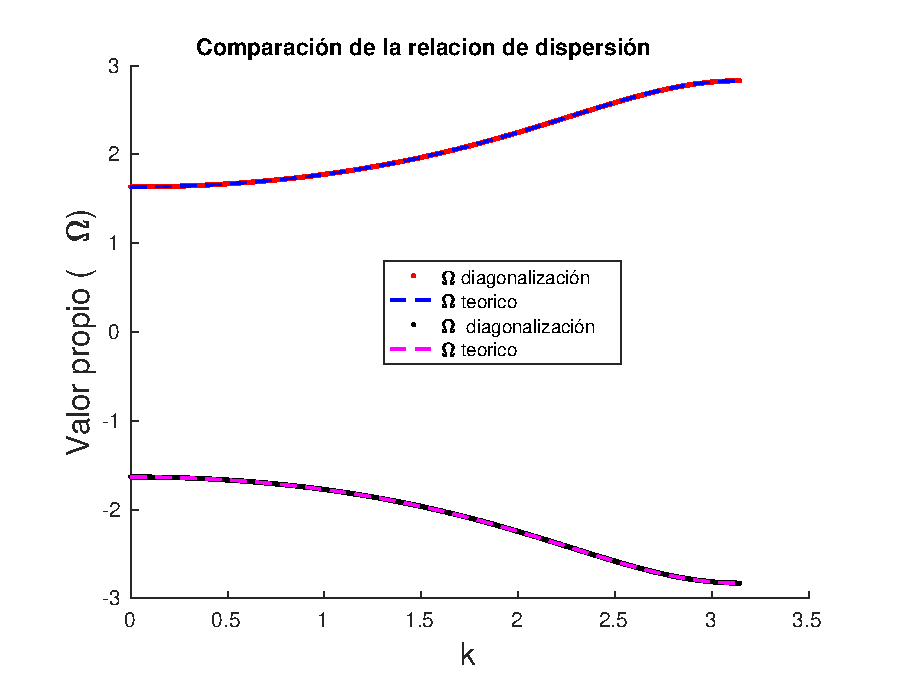
\includegraphics[scale=0.46]{RDSP-E.eps}}
\caption{Relacion de dispersion y comparacion para un set de parametros $\lambda=0.25$ $\omega_{o}=2$ y $\chi=0.3$.}
\end{figure}
\par 
Posteriormente, con la región de valores propios ($\Omega$) para las soluciones no lineales delimitada (gap), se procedió a determinar las soluciones estacionarias del sistema para N=2 y N=101, es decir, resolver u obtener las raíces del sistema de N ecuaciones planteado en ($8$), aplicando el método de Newton-Raphson, mediante la función \textit{fslove()} de MATLAB. Para tres diferentes casos en los que se introdujo en la función \textit{fsolve} la semilla simétrica, antisimétrica y asimétrica respectivamente. Siendo la simétrica todos los resonadores con amplitud cero y solo los dos del medio con amplitud $1$. En la antisimetrica los dos del medio con amplitud $-1$ y en la asimétrica, solo el resonador del medio con amplitud $1$.\\
\begin{figure}[h!]
\centering
\subfigure[] {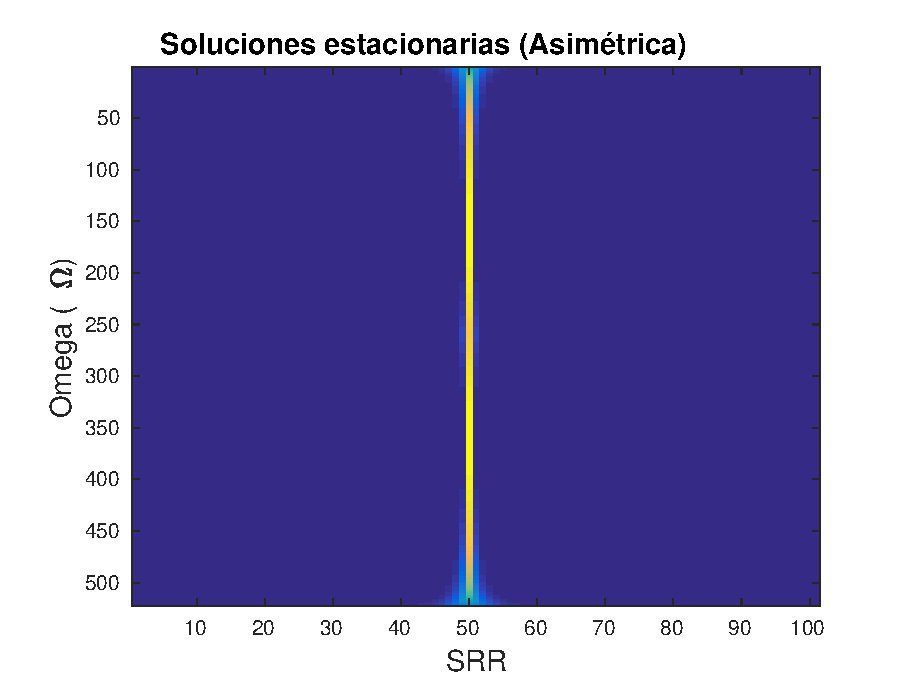
\includegraphics[scale=0.48]{SE1011.eps}}
\subfigure[] {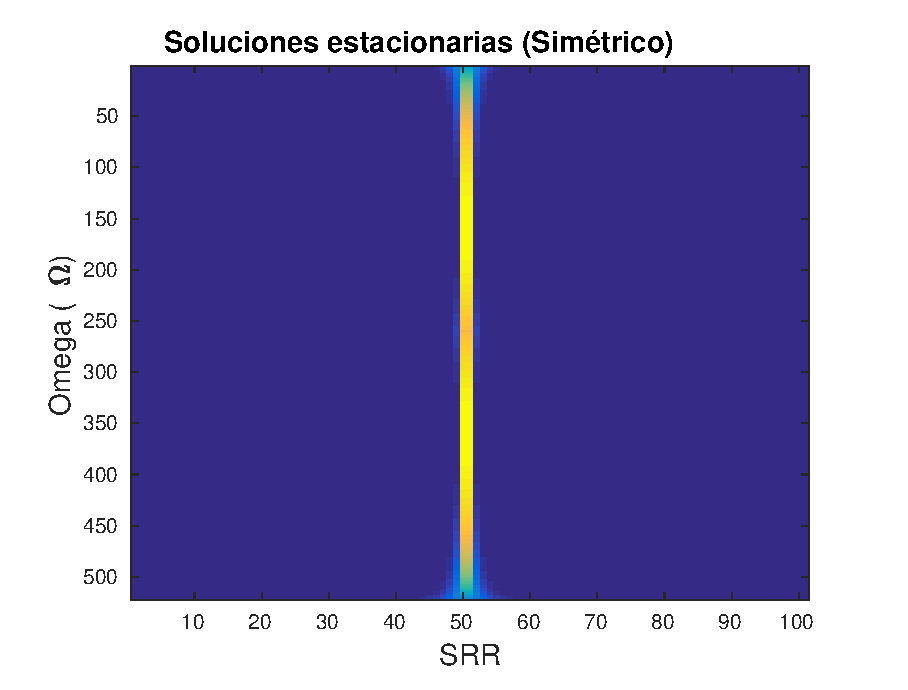
\includegraphics[scale=0.48]{SE1012.eps}}
\caption{Soluciones estacionarias para $a)$ 2 y $b)$ 101 resonadores, para un set de parametros $\lambda=0.25$ $\omega_{o}=2$ y $\chi=0.3$.}
\end{figure}
\par 
Las cuales fueron caracterizadas mediante su hamiltoniano (ecuacion $3$ ), el cual solo depende de $V_{n}$ ya que al ser estacionarias, $\dot{q}_{n}$ es cero. Esta caracterizacion perimitio observar las familias de soluciones para las diferentes semillas en funcion de $\Omega$, tanto para N=2 cómo para N=101, cómo se visualiza en la figura ($4$).
\begin{figure}[h!]
\subfigure[] {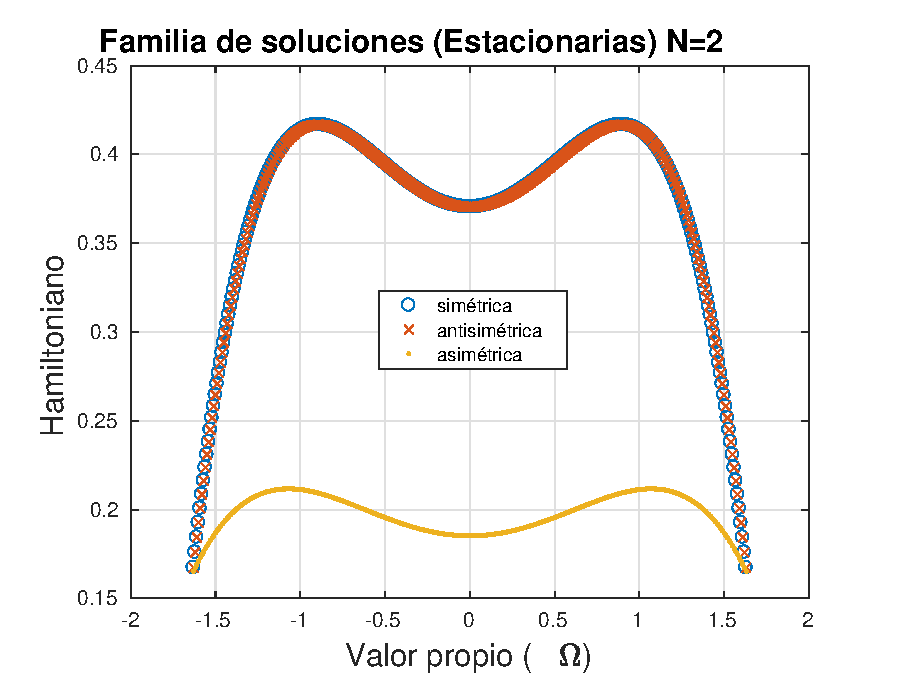
\includegraphics[scale=0.48]{FS-2.eps}}
\subfigure[] {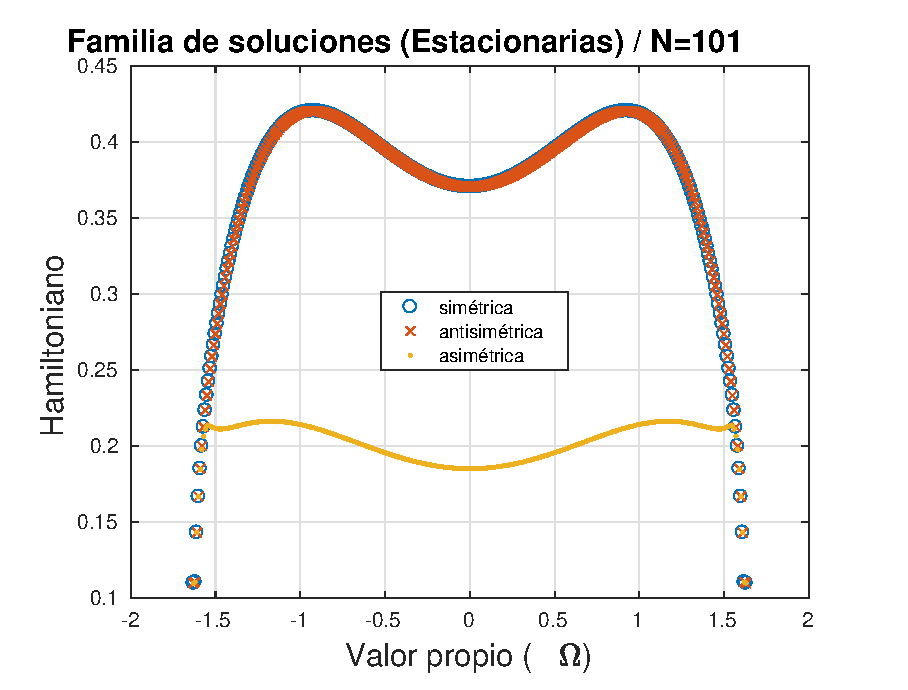
\includegraphics[scale=0.48]{FS-N.eps}}
\caption{Familia de soluciones a) Simetrico y b) asimetrico. }
\end{figure}
\par 
Donde se observa que la solución simétrica y antisimetrica presentan el mismo comportamiento, ya que estas son análogas y lo que las diferencia son el signo de su amplitud, el cual deja de tomar importancia en este caso debido a los términos cuadráticos en el potencial. De igual forma también se visualiza como las tres familias (soluciones) toman valores similiares a medida que se acercan sus valores propios a la zona lineal. Con el fin de observar como cambian las soluciones de ambas familias (simétrica y asimétrica), se graficaron algunas soluciones para diferentes valores de $\Omega$ acercándose a la zona lineal cómo se visualiza en la figura ($5$), donde se aprecia que las soluciones estacionarias del sistema son localizadas, y toman valores cercanos a cero cuando el valor propio tiende hacia la zona lineal, es decir fuera del gap.
\begin{figure*}[http]
\centering
\subfigure[] {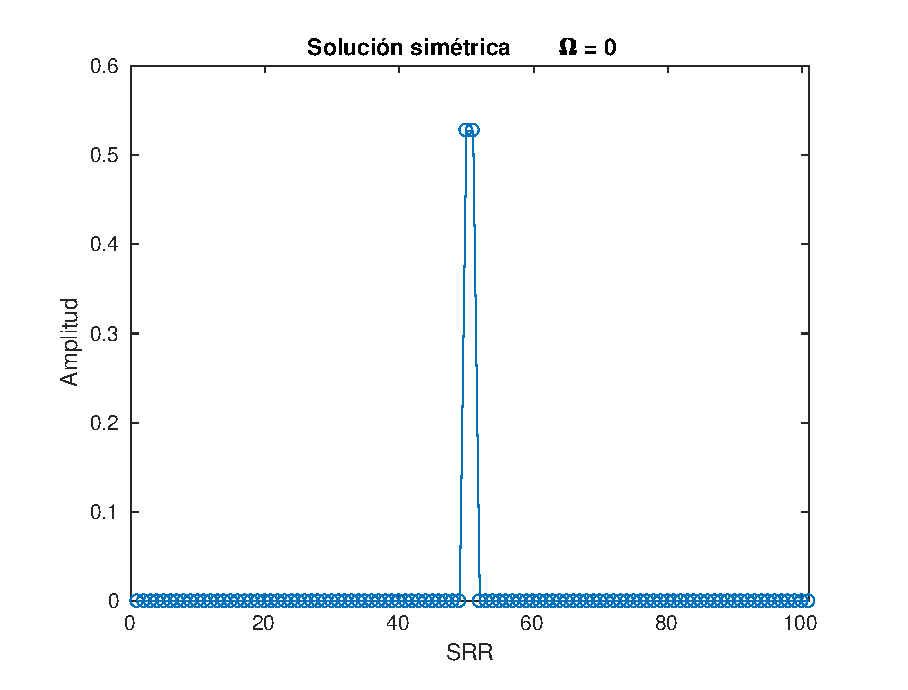
\includegraphics[scale=0.45]{SS-0.eps}} \subfigure[] {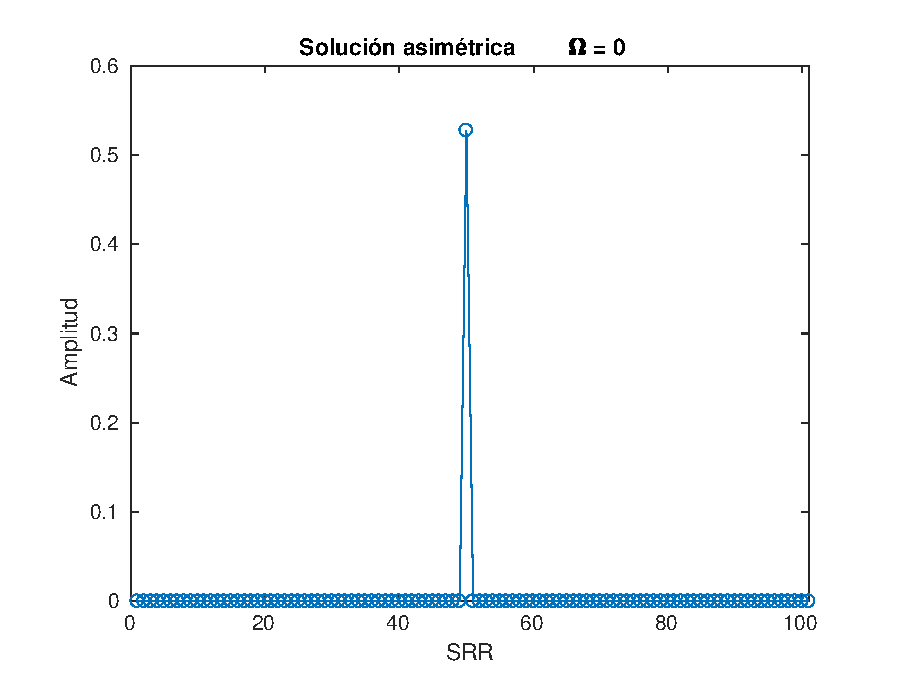
\includegraphics[scale=0.45]{SA-0.eps}}\\
\subfigure[] {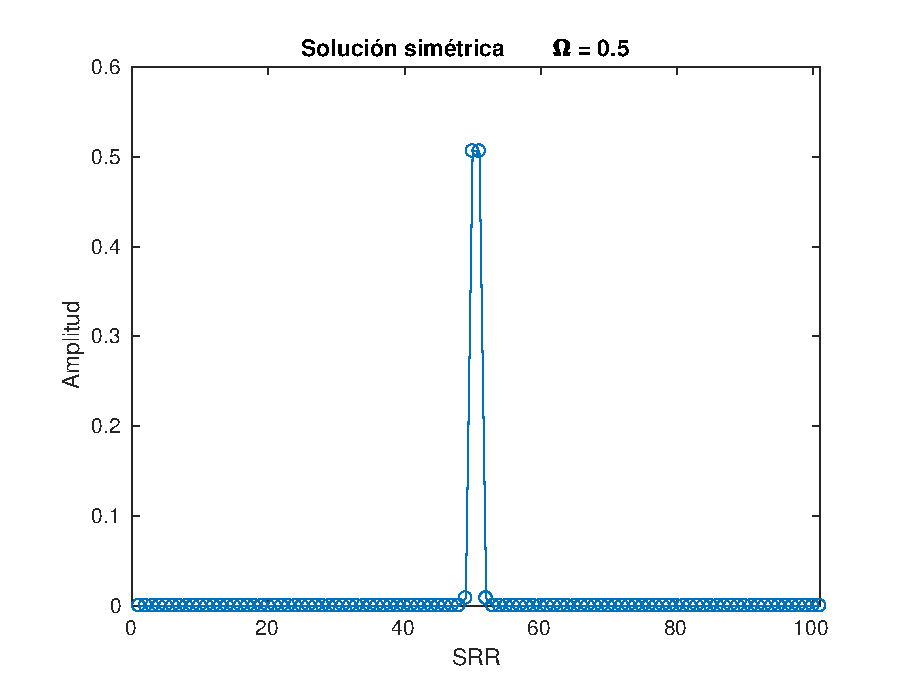
\includegraphics[scale=0.45]{SS-05.eps}} \subfigure[] {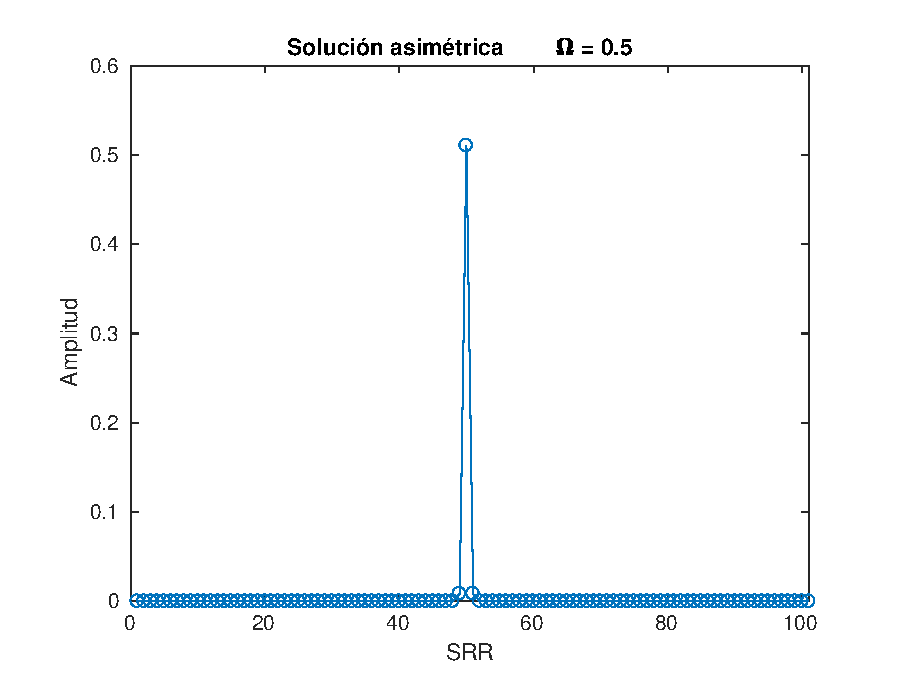
\includegraphics[scale=0.45]{SA-05.eps}}\\
\subfigure[] {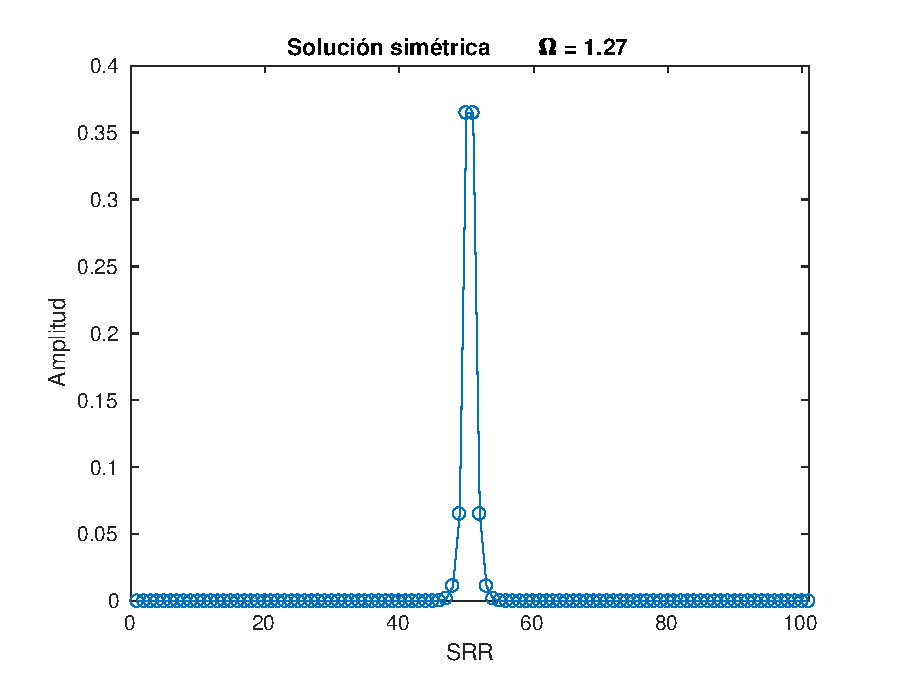
\includegraphics[scale=0.45]{SS-127.eps}} \subfigure[] {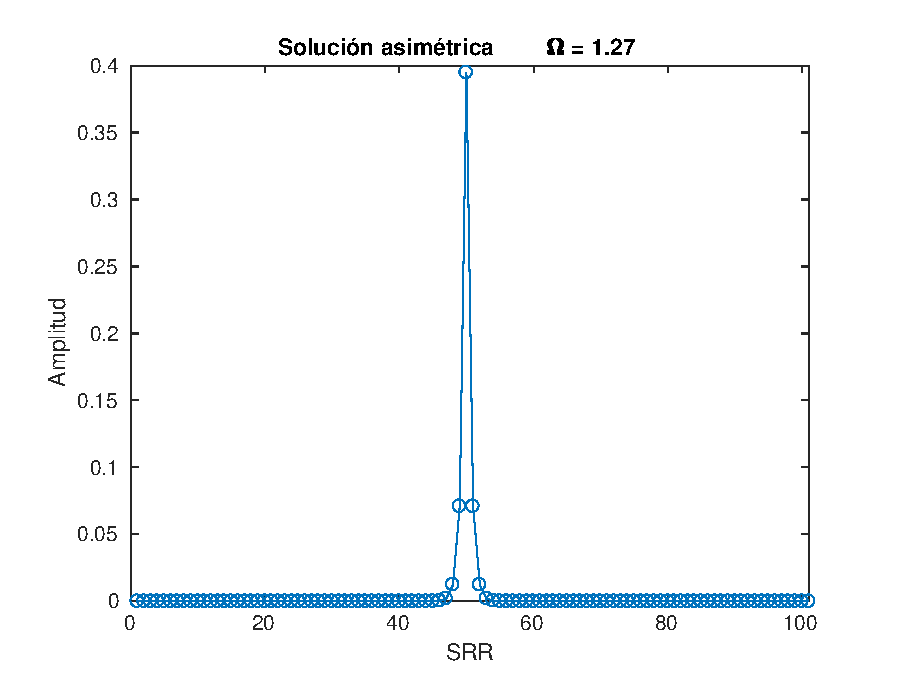
\includegraphics[scale=0.45]{SA-127.eps}}\\
\subfigure[] {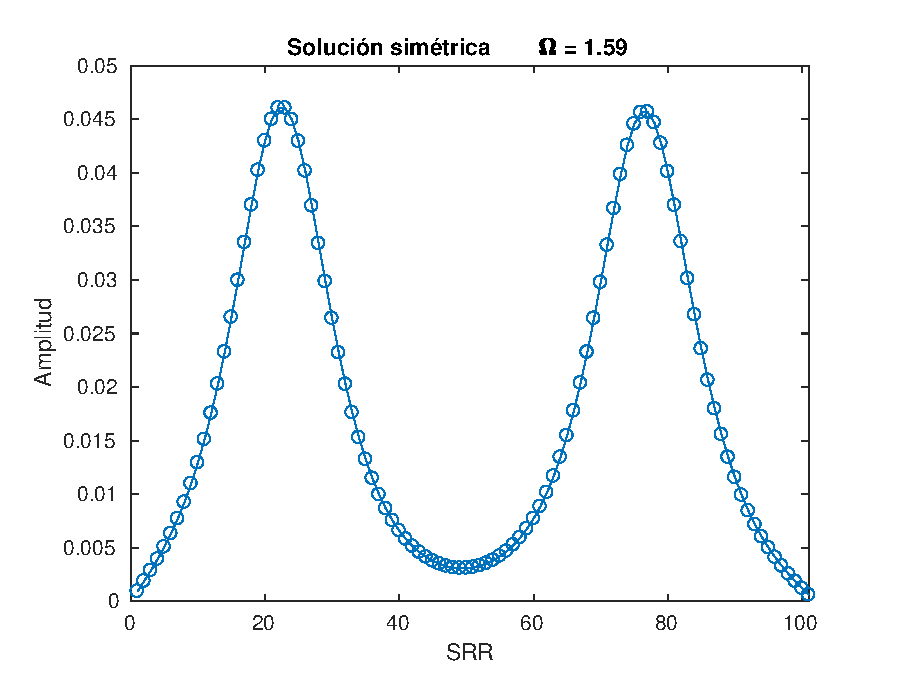
\includegraphics[scale=0.45]{SS-159.eps}}\subfigure[] {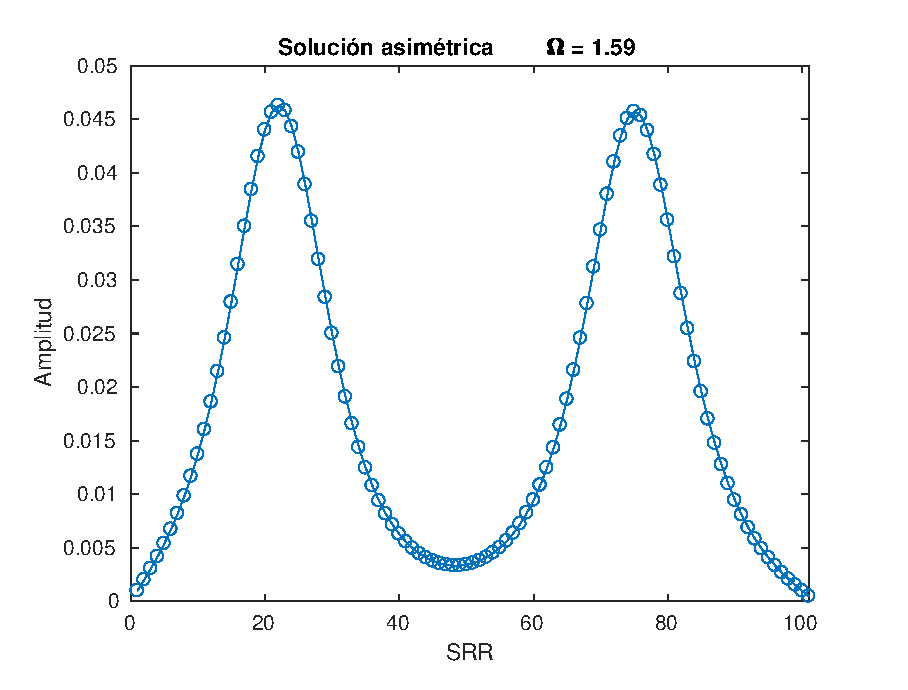
\includegraphics[scale=0.45]{SA-159.eps}}\\
\caption{Soluciones localizadas}
\end{figure*}
\par 
Posteriormente, se procedió a propagar las soluciones estacionarias simétrica y asimétrica encontradas para un valor especifico de $\Omega$. Mediante el modelo plateado en la ecuación 11. Para realizar la propagación, en primera instancia se estableció el intervalo de tiempo de estudio, y las condiciones dinámicas iniciales del sistema $(q_{o},\dot{q}_{o})$; las cuales seran las soluciones estacionarias y todas las $\dot{q}_{n}$ cero. Luego se transformo el sistema de ecuaciones diferenciales de segundo orden de la ecuación 11, en dos sistemas de ecuaciones diferenciales de primer orden, y finalmente utilizando el Runge kutta de cuarto orden de MATLAB mediante la función \textit{ode45()}, fue posible calcular cada una de las cargas ($q_{n}$) y  $\dot{q}_{n}$,  acumuladas en cada condensador después de un tiempo $t_{f}$ transcurrido desde la perturbación inicial, cómo se aprecia en la figura ($6$).\\
\begin{figure}[h!]
\centering
\subfigure[] {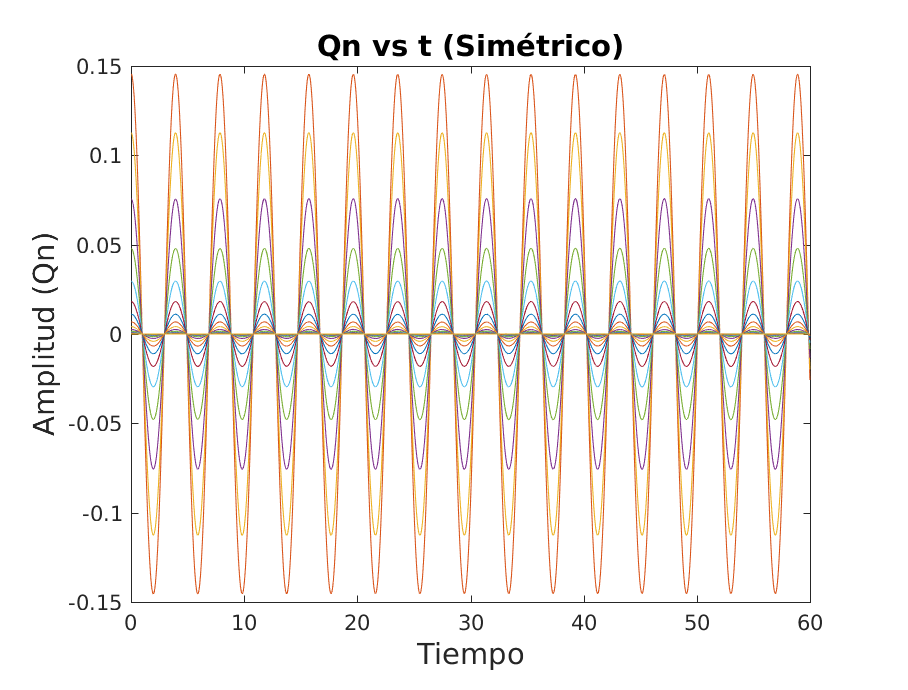
\includegraphics[scale=0.5]{QvstS.eps}} 
\subfigure[] {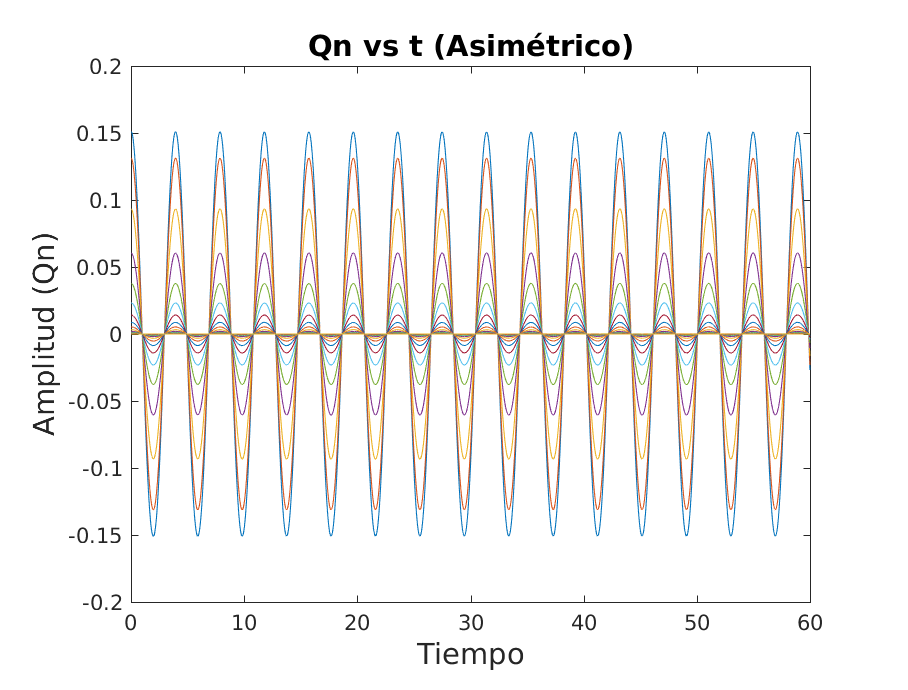
\includegraphics[scale=0.5]{QvstA.eps}}
\caption{Carga en funcion del tiempo en cada SRR'S para la forma de la solución a) simétrico b) asimétrico. N=100 con set de parámetros $\lambda=0.25$ $\Omega=1.2$ $\omega_{o}=2$ y $\chi=0.3$.}
\end{figure}
\par 
Ya que no hay disipación o conducciones externas, la energía del sistema (ecuación 3) se debe conservar, cómo se observa en la figura $7$, la cual presenta las energías cinéticas y potencial ($V_{n}$) en función del tiempo, y la energía total del sistema es decir el hamiltoniano, el cual es una constante.
\begin{figure}[h!]
\centering
\subfigure[] {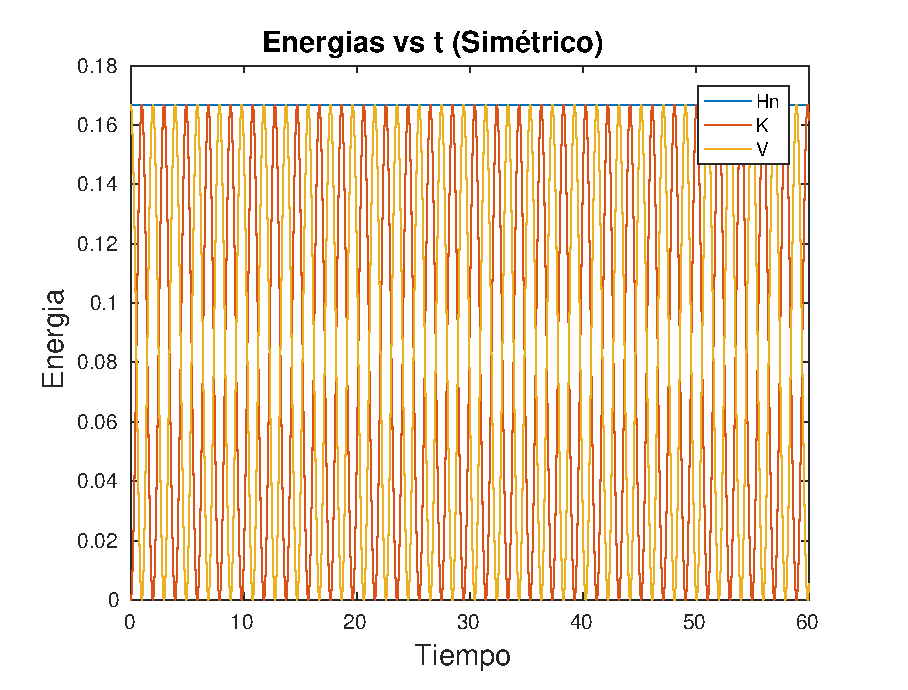
\includegraphics[scale=0.5]{EvstS.eps}} 
\subfigure[] {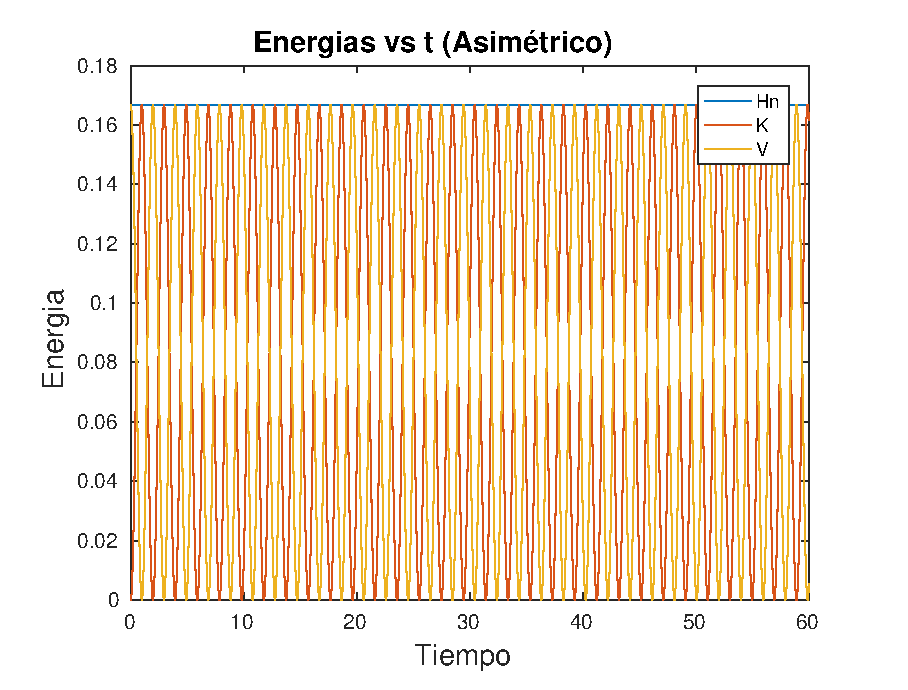
\includegraphics[scale=0.5]{EvstA.eps}}
\caption{Energias para las soluciones a) simétrica y b) asimétrica de la figura 6.}
\end{figure}
\par 
En el perfil de las propagaciones figura $8$ a) y c) , se aprecia como es el intercambio de carga entre los resonadores para cada tipo de familia, donde se observa que la solución se mantiene localizada en el tiempo. Con la intención de dilucidar cómo afecta el intercambio de cargas a los resonadores vecinos de la solución localizada,  durante la propagación de la solución estacionaria, se obtuvieron los valores absolutos de las cargas en función del tiempo utilizando la función \textit{abs()}, y nuevamente utilizando la función \textit{imagesc()} se graficaron éstos valores, donde observa en la figura $8$ b) y d), el rango de acción y como la perturbación central afecta sus vecinos.\\
\begin{figure}[h!]
\centering
\subfigure[] {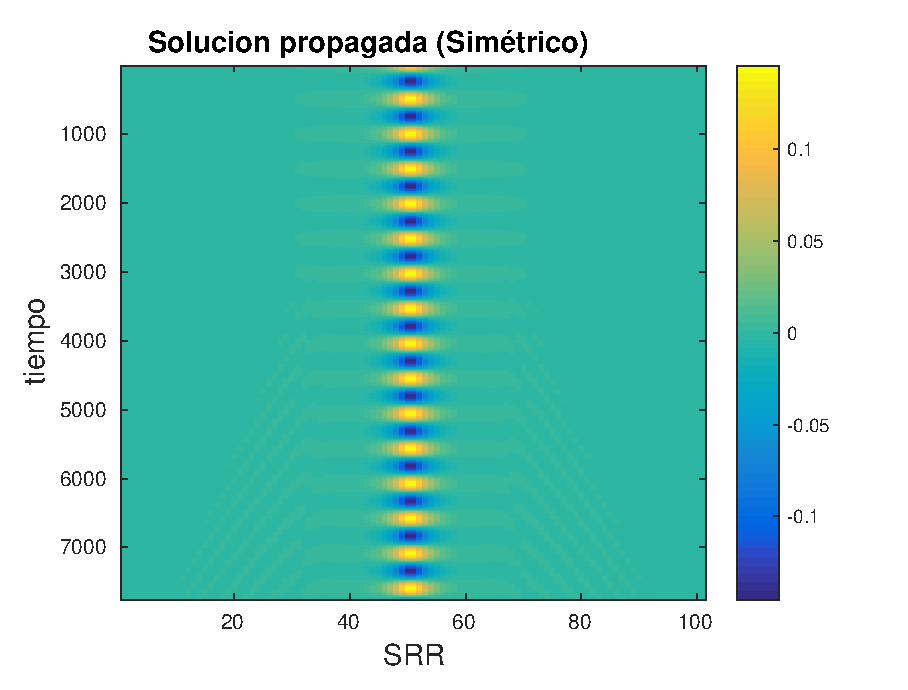
\includegraphics[scale=0.41]{SPS.eps}} 
\subfigure[] {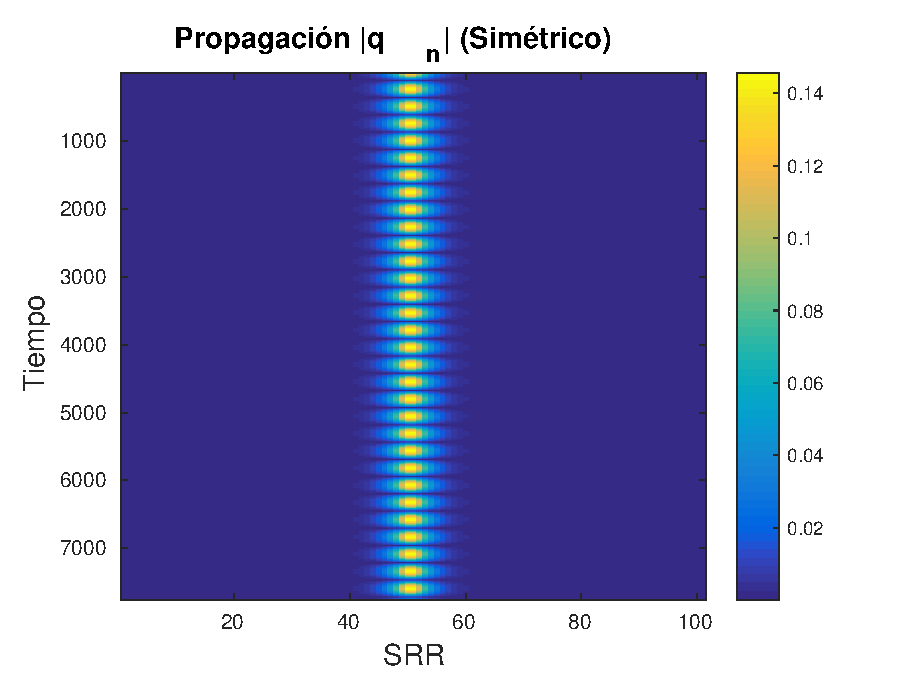
\includegraphics[scale=0.41]{SPS2.eps}}
\subfigure[] {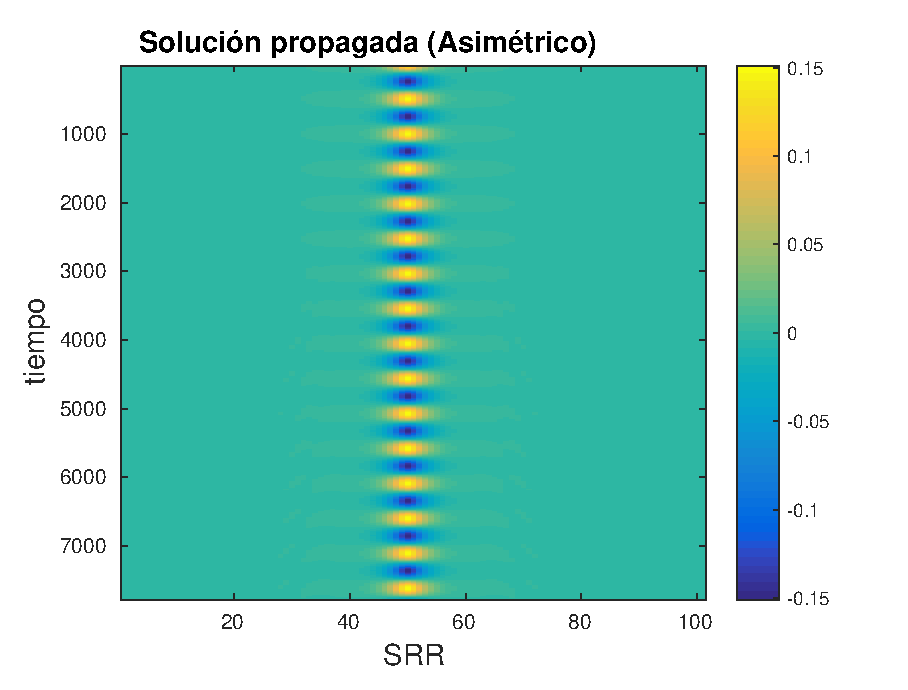
\includegraphics[scale=0.41]{SPA.eps}} 
\subfigure[] {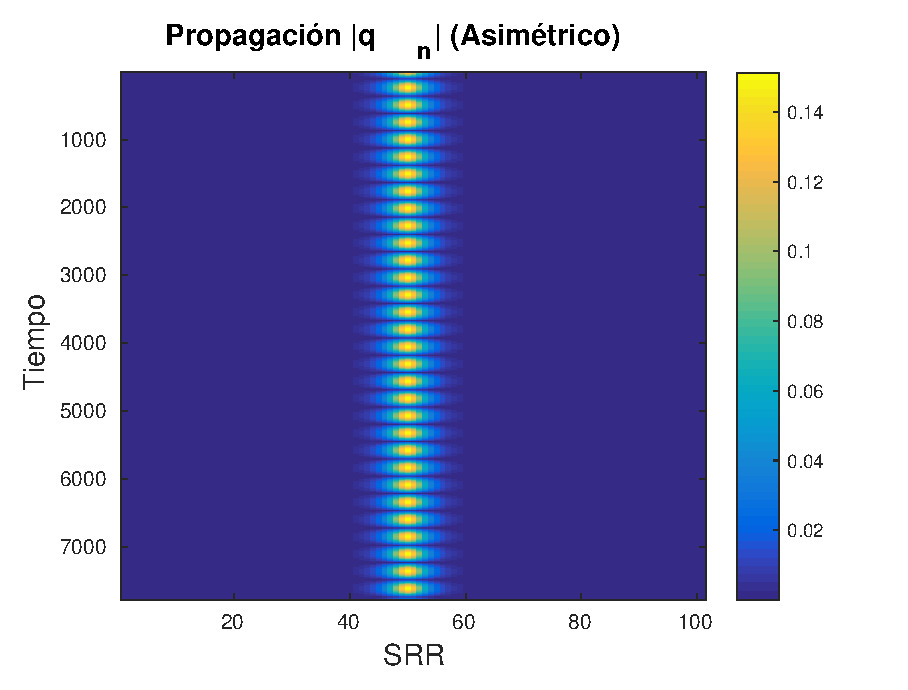
\includegraphics[scale=0.41]{SPA2.eps}}
\caption{Perfil de la propagación a) simétrico y c) asimétrico. Valor absoluto de la propagación b) simétrico y d) asimétrico.}
\end{figure}
\section*{\normalsize{CONCLUSIÓN}}
Mediante las herramientas computacionales de MATLAB, se pudo estudiar y analizar el comportamiento del modelo no lineal simplificado de un arreglo unidimensional de N resonadores de anillo dividido (SRR\textquotesingle S), comprobando que el método de diagonalizacion es análogo a la ecuación teórica de la relación de dispersión, para la determinación de los valores propios del sistema, tanto lineales cómo no lineales. De igual forma se determinaron las soluciones estacionarias para diferentes semillas utilizando el metodo de Newton-Raphson, encontrando que las soluciones del problema no lineal son localizadas. Mediante el hamiltoniano en funcion del valor propio, se obtuvieron las familias de soluciones para un sistema de N=2 y N=101 SRR\textquotesingle S. Posteriormente se propago las soluciones estacionarias simétrica y asimétrica, encontrando que las soluciones se mantienen localizadas en el tiempo y debido a la ausencia de efectos disipativos o conducciones externas, la energía del sistema se conserva, y como se ven afectos los resonadores vecinos a la solución localizada en ambos casos. 
\section*{Referencias} 
\begin{itemize} 
\item[[ 1]] Rev. Acad. Colomb. Cienc. Ex. Fis. Nat. 40(156):395-401, julio-septiembre de 2016doi: http://dx.doi.org/10.18257/raccefyn.345

\item[[ 2]] S. Linden, et al., IEEE J. Selec. Top. Quant. Electron. 12 (2006) 1097.
\item[[ 3]] V.M. Shalaev, Nat. Photon. 1 (2007) 41.
\item[[ 4]] C.M. Soukoulis, S. Linden, M. Wegener, Science 315 (2007) 47.
\item[[ 5]] M. Kafesaki, et al., Physica B 394 (2007) 148.
\item[[ 6]] T.J. Yen, et al., Science 303 (2004) 1494.
\item[[ 7]] N. Katsarakis, et al., Opt. Lett. 30 (2005) 1348.
\item[[ 8]] Breathers in one-dimensional binary metamaterial models N. Lazarides, M.I. Molina, G.P. Tsironis. 
\item[[ 9]] N. Engheta and R. W. Ziolkowski, eds. Electromagnetic Metamaterials: Physics and Engineering Explorations
(Wiley-IEEE Press, 2006), 440 pp.
\item[[ 10]]D. A. Powell, M. Lapine, M. V. Gorkunov, I. V. Shadrivov, and Yu. S. Kivshar, “Metamaterial tuning by manip-
ulation of near-field interaction,” Phys. Rev. B 82, 155128 (2010).
\item[[ 11]]  M. Gorkunov, M. Lapine, E. Shamonina, and K. H. Ringhofer, “Effective magnetic properties of a composite
material with circular conductive elements,” Eur. Phys. J. B 28, 263–269 (2002).
\item[[ 12]]Discrete dissipative localized modes in nonlinear magnetic metamaterials Nikolay N. Rosanov, Nina V. Vysotina, Anatoly N. Shatsev, Ilya V. Shadrivov, David A. Powell, Yuri S. Kivshar.
\item[[ 13]]Gay-Balmaz, Philippe; Martin, Olivier J. F. (2002). "Electromagnetic resonances in individual and coupled split-ring resonators". Journal of Applied Physics. 92 (5): 2929. Bibcode:2002JAP....92.2929G. doi:10.1063/1.1497452.

\item[[ 14]] T.H. Hand, S.A. Cummer, J. Appl. Phys. 103 (2008) 066105.
\item[[ 15]] I.V. Shadrivov, A.B. Kozyrev, D. van der Weide, Yu.S. Kivshar, Appl. Phys. Lett.
93 (2008) 161903.
\item[[ 16]]D.A. Powell, I.V. Shadrivov, Yu.S. Kivshar, M.V. Gorkunov, Appl. Phys. Lett. 91
(2007) 144107.
\item[[ 17]] B. Wang, J. Zhou, T. Koschny, C.M. Soukoulis, Opt. Express 16 (2008)
16058.
\item[[ 18]]N. Lazarides, M. Eleftheriou, G.P. Tsironis, Phys. Rev. Lett. 97 (2006) 157406.
\item[[ 19]]M. Eleftheriou, N. Lazarides, G.P. Tsironis, Phys. Rev. E 77 (2008) 036608.
\item[[ 20]]I.V. Shadrivov, A.A. Zharov, N.A. Zharova, Yu.S. Kivshar, Photon. Nanostruct.
Fund. Appl. 4 (2006) 69.

\item[[ 21]] M.I. Molina, N. Lazarides, G.P. Tsironis, Bulk and surface magnetoinductive
breathers in binary metamaterials, Phys. Rev. E 80 (2009) 046605.
\end{itemize}
\subsection*{Anexos}

\begin{lstlisting}
1. Codigo en MATLAB para 
la parte lineal. 
N=1000; la=0.25; wn= 2; 
k=linspace(0,pi,N); zi=0.3; 

%PARTE LINEAL
om= (wn)./(sqrt(1+2*la*cos(k)));
 om2=-om; 

%LA MATRIZ DE AUTOVALORES (LINEAL)
a= la*ones(1,N-1); b=ones(1,N); 
M= diag(a,-1) + diag(b,0) + diag(a,1) 
; M(1,N)=la ; M(N,1)=la; Minv=inv(M); 

W=(wn.^2).*Minv; 

eigen=sqrt(eig(W));
 
% PARTE NO LINEAL
function f=sistemaqn(x,wo,omega,zi,la)
a= -la*(omega.^2); b= (wo.^2 -omega.^2);
 c=-(3/4)*zi* wo.^6; 

W3= b.*ones(1,length(x)) + c*(x.^2); 
W1= a*ones(1,length(x)-1); 

M=diag(W1,1) + diag(W3,0) + diag(W1,-1);

f=M*x(:); 
end

x01=x0; x02=x0; qn1=[];
con=[] ; qn2=[]; con2=[] ; 

options = optimoptions(
'fsolve','Display','off');

for i=1:length(omega)
fun=@(x) sistemaqn(x,wn,
omega(i),zi,la) ; 
[xx,yy]=fsolve(fun,x01,options); 
qn1=[qn1;xx];   
x01=[qn1(i,:)];
    
fun2=@(x) sistemaqn(x,wn
,-omega(i),zi,la) ; 
[xx2,yy2]=fsolve(fun2,x02,options); 
qn2=[qn2;xx2];                         
con2=[con2;sum(yy2.^2)];      
x02=[qn2(i,:)];
end

f= [flipud(qn2);qn1]; 
end

%PROPAGACION

x0= qn(m,:); 
x0=x0(:); 
v0=zeros(N_q,1); 
X0=[x0;v0]; 
tf=60; 
%Evolucion del sistema
options=odeset('RelTol'
,1e-10,'Abstol',1e-10);
[t,y]=ode45(@(t,X) 
propagar(t,X,zi,wn,la),
[0 tf],X0,options);

Qn=y(:,1:N_q); 
Qnv=y(:,N_q+1:2*N_q); 

%%% HAMILTON
DI= 0.5*[(Qnv(:,1).^2 + l
a*Qnv(:,1).*Qnv(:,2)) ,
Qnv(:,2:N_q-1).^2 + 
la*Qnv(:,2:N_q-1).*( 
Qnv(:,1:N_q-2) + Qnv(:,3:N_q) ),
Qnv(:,N_q).^2 + 
la*Qnv(:,N_q).*Qnv(:,N_q-1)]; 
 
VI= 0.5*wn.^2 .*Qn.^2 .*(
 1 - 0.5*zi*wn.^2.*(wn.*Qn).^2);  }
HN=DI+VI; 
hj=sum(HN,2); 
di= sum(DI,2); vi=sum(VI,2); 
\end{lstlisting}

\end{document}
